% =============================================================
%  System Calculation — calculation procedures of the load flow
%  framework hvdc_lf (MMC VSC HVDC, station and point-to-point link).
%  Uses the shared American Terawatt report style.
%  Worked examples: tables and figures are generated by the scripts
%  in <chapter>/fig/ from the example data in tools/example_data.py
%  (hvdc_lf 0.52.0); run them from this folder before building.
%  Compile:  latexmk -xelatex system_calc.tex
% =============================================================
\documentclass[11pt,a4paper]{article}

\usepackage[corporate]{../../template/attemplate}
\usepackage{placeins}
\usepackage{longtable}

% ---- Report metadata ----------------------------------------
\reporttitle{System Calculation}
\reportsubtitle{Calculation procedures of the load flow of an MMC VSC HVDC station and link}
\atEyebrow{System Calculation}

\reportauthor{Eugen Starschich}
\reportdocnumber{ATW-REP-SYC-001}
\reportrevision{0.1}
\reportstatus{Draft}
\reportdate{\today}
\reportconfidentiality{Internal}

% table rows generated by the chapter scripts: primitive \input, so that a rule may follow
\makeatletter
\newcommand{\tablerows}[1]{\@@input #1.tex }
\makeatother

% values of the worked examples, generated by the chapter scripts
% generated by station_example.py with hvdc_lf 0.52.0; do not edit by hand
\newcommand{\exPdc}{$-$984.61}
\newcommand{\exId}{1.2308}
\newcommand{\exLoss}{15.394}
\newcommand{\exEta}{98.461}
\newcommand{\exM}{0.8679}
\newcommand{\exUconv}{400.062}

% generated by converter_example.py with hvdc_lf 0.52.0; do not edit by hand
\newcommand{\cvUv}{421.33}
\newcommand{\cvQ}{148.3}
\newcommand{\cvUdc}{800.12}
\newcommand{\cvP}{$-$990.91}
\newcommand{\cvIrms}{0.7997}
\newcommand{\cvIpk}{1.3811}

% generated by thermal_example.py with hvdc_lf 0.52.0; do not edit by hand
\newcommand{\thTout}{55.61}
\newcommand{\thPplate}{3.859}
\newcommand{\thTjmax}{77.5}
\newcommand{\thHot}{D2}
\newcommand{\thArm}{upper}

% generated by link_example.py with hvdc_lf 0.52.0; do not edit by hand
\newcommand{\lkRtwenty}{2.160}
\newcommand{\lkRseventy}{2.584}
\newcommand{\lkUinv}{396.819}
\newcommand{\lkId}{1.2308}
\newcommand{\lkLine}{7.830}
\newcommand{\lkLoss}{37.920}
\newcommand{\lkEta}{96.208}


\begin{document}

\makecover

\revisionhistory{
  \revrow{0.1}{Nov. 19, 2026}{Eugen Starschich}{Initial document: station, converter, semiconductor and cooling, DC line, link, verification}
}

\newpage
\tableofcontents
\clearpage

% ---- Body ---------------------------------------------------
\section{Abbreviations}
\label{sec:abbreviations}

\begin{longtable}{@{}l p{0.80\linewidth}@{}}
  \toprule
  \multicolumn{1}{c}{\textbf{Abbreviation}} & \textbf{Meaning} \\
  \midrule
  \endhead
  AC    & Alternating current \\
  DC    & Direct current \\
  HVDC  & High-voltage direct current \\
  IEC   & International Electrotechnical Commission \\
  IGBT  & Insulated-gate bipolar transistor \\
  MMC   & Modular multilevel converter \\
  OHL   & Overhead line \\
  PCC   & Point of common coupling \\
  RFC   & Relaxed field of cathode (diode technology of the IGBT module) \\
  RMS   & Root mean square \\
  SM    & Submodule \\
  VSC   & Voltage-sourced converter \\
  XLPE  & Cross-linked polyethylene \\
  \bottomrule
\end{longtable}

% =============================================================
%  Symbols
%  Collects the symbols of Sections 4 to 9. Compound subscripts use
%  an underscore (U_{dpe\_rec}); complex quantities are underlined.
% =============================================================
\section{Symbols}
\label{sec:symbols}

AC voltages are line-to-line RMS values unless stated otherwise; DC voltages are pole-to-ground. Complex quantities
are underlined. Powers and currents carry the sign of the convention of Section~\ref{sec:conventions}.

\begin{longtable}{@{}l p{0.80\linewidth}@{}}
  \toprule
  \multicolumn{1}{c}{\textbf{Symbol}} & \textbf{Description} \\
  \midrule
  \endhead
  $a$        & Inner modulation index of the converter \\
  $B$        & Shunt susceptance of the AC line \\
  $C$        & Capacitance; $C'$ per unit length of the AC line, $C_{sm}$ of one submodule \\
  $c_p$      & Specific heat capacity of the cooling water \\
  $e$, $\underline{E}$ & Internal converter voltage (phase) behind the arm reactors; $e_3$ the third harmonic \\
  $E_{on}$, $E_{off}$, $E_{rec}$ & Turn-on, turn-off and reverse-recovery energy per pulse \\
  $f$        & Frequency; $f_r$ rated frequency, $f_{sw}$ average switching frequency of a submodule \\
  $I$        & Current; $I_d$ DC current of a pole, $I_{arm}$ arm current, $I_C$ rated collector current \\
  $i_0$      & No-load current of the transformer \\
  $k$        & DC voltage across one converter in multiples of $U_{dpe}$ \\
  $k_3$      & Peak factor of the arm voltage, 1 or $\sqrt{3}/2$ with third harmonic injection \\
  $L$        & Inductance; $L_{arm}$ of one arm reactor \\
  $l$        & Length of a line \\
  $m$        & Modulation index of the converter \\
  $N$        & Submodules per arm \\
  $n$        & Voltage ratio of the transformer; $n_{conv}$ converters per station, $n_{par}$ modules in parallel,
               $n_{ins}$ inserted submodules \\
  $P$, $Q$, $\underline{S}$ & Active, reactive and complex power \\
  $P_{cu}$, $P_{fe}$ & Load and no-load losses of the transformer \\
  $Q_w$      & Cooling water flow per cold plate \\
  $R$        & Resistance; $R'$ per unit length \\
  $R_{th}$   & Thermal resistance; $R_{th\_jc}$ junction to case, $R_{th\_cs}$ case to heat sink, $R_{th\_hw}$ heat
               sink to water \\
  $r$        & Slope resistance of the on-state model \\
  $T$        & Temperature; $T_j$ junction, $T_w$ water \\
  $u_k$      & Short-circuit voltage of the transformer \\
  $U$        & Voltage; $U_{dpe}$ DC voltage pole-to-ground at the station DC terminal, $U_{dc}$ across the
               converter, $U_{conv}$ internal converter voltage \\
  $u_{sm}$, $u_c$ & Average and instantaneous capacitor voltage of a submodule \\
  $v_0$      & Threshold voltage of the on-state model \\
  $W$        & Energy stored in the submodule capacitors of an arm; $W_0$ its average \\
  $X$        & Reactance \\
  $Z$        & Impedance; $Z_{th}$ transient thermal impedance \\
  $\alpha$   & Temperature coefficient of the conductor resistance \\
  $\rho$     & Density of the cooling water \\
  $\tau$     & Time constant of a Foster element \\
  $\omega$   & Angular frequency, $2 \pi f$ \\
  \bottomrule
\end{longtable}

% =============================================================
%  Introduction: scope, structure of the calculation, conventions,
%  example data.  Sources: [1] hvdc_lf repository.
% =============================================================
\section{Introduction}
\label{sec:introduction}

This report describes the calculation procedures of the steady-state load flow of a voltage-sourced converter
(VSC) HVDC transmission with modular multilevel converters (MMC), as implemented in the load flow framework
\texttt{hvdc\_lf}~[1]. It states for every element the model, the equations and the order in which they are
solved, for a single converter station and for a point-to-point link of two stations. The procedures refer to
\texttt{hvdc\_lf} 0.52.0; every number of the worked examples is produced by the scripts named in the chapter
header comments from the example data of Section~\ref{sec:example-data}.

\subsection{Structure of the calculation}
\label{sec:structure}

The calculation has three levels:

\begin{itemize}
  \item \textbf{Components.} AC network at the point of common coupling (PCC), AC line, converter transformer,
        converter with its arm reactors and its semiconductor, DC reactor, DC line. Each component has a data model
        and one or more calculation methods; the method of a component is part of its data.
  \item \textbf{Station.} The components of one station, calculated in a chain from the PCC to the station DC
        terminal (Section~\ref{sec:station}).
  \item \textbf{Link.} Two stations and the DC line between their DC terminals (Section~\ref{sec:link}).
\end{itemize}

The data of a calculation fall into three groups: the component data (design values, stored once per version in
the component catalogue), the configuration (which components form a station or a link, and its topology) and the
operating point (case). Values that change with the operation of the system --- active and reactive power, PCC
voltage, frequency, tap position, DC voltage, auxiliary power demand, cooling water temperature and flow --- belong
to the operating point and not to the components. A configuration holds no operating values.

The topology sets two factors: $n_{conv}$, the converters per station, and $k$, the DC voltage across one converter
in multiples of the pole-to-ground voltage $U_{dpe}$. A symmetrical monopole has $n_{conv} = 1$, $k = 2$; a bipole
has $n_{conv} = 2$, $k = 1$. Both topologies carry the DC current $I_d$ in two pole conductors, and
$n_{conv} \cdot k = 2$. The worked examples use a symmetrical monopole.

\subsection{Sign convention and units}
\label{sec:conventions}

Active power, reactive power and current are positive in the direction towards the AC grid, at every port of a
station and on the AC and the DC side alike:

\begin{itemize}
  \item a rectifier has $P < 0$ at its PCC and at its DC terminal, an inverter $P > 0$ at both;
  \item $Q > 0$ is reactive power supplied by the station to the AC grid;
  \item losses are positive: the loss of an element is the power at its grid-side port minus the power at its other
        port, both in this convention, e.g.\ $P_{loss\_cv} = P_{dc} - P_{ac}$ for the converter.
\end{itemize}

The operating mode of a station is not part of its data. The sign of the given active power decides whether it
works as rectifier or inverter, and for a link which station is the rectifier.

The units are metric: kV, kA, MW, Mvar, MV$\cdot$A, $\Omega$, mH, mF, km, $^{\circ}$C, l/min. AC voltages are
line-to-line RMS values, DC voltages pole-to-ground unless stated as the voltage across a converter. With kV and kA,
$\mathrm{kV} \cdot \mathrm{kA} = \mathrm{MW}$ and $\mathrm{kA}^2 \cdot \Omega = \mathrm{MW}$; with V and kA,
$\mathrm{V} \cdot \mathrm{kA} = \mathrm{kW}$.

\subsection{Example data}
\label{sec:example-data}

The worked examples use one station design, given in Table~\ref{tab:example-data}; the link joins two stations of this
design by a 300\,km cable (Section~\ref{sec:dc-line}). The data are placeholders except the semiconductor, which is
the module of the datasheet~[2]. The station operating point is $U_{pcc} = 345$\,kV, $P_{pcc} = -1000$\,MW (rectifier),
$Q_{pcc} = 0$, tap 0, $U_{dpe} = 400$\,kV and 500\,kW auxiliary power.

\begin{table}[!ht]
  \centering
  \small
  \begin{tabularx}{\linewidth}{@{}l >{\raggedright\arraybackslash}X@{}}
    \toprule
    \textbf{Component} & \textbf{Data} \\
    \midrule
    AC network      & 345\,kV, 60\,Hz, voltage band 0.90 to 1.10\,pu \\
    AC line         & 40\,km OHL, 2 circuits, nominal $\pi$; per circuit $R' = 0.075\,\Omega$/km per sub-conductor,
                      2 sub-conductors, $X' = 0.360\,\Omega$/km, $C' = 12.5$\,nF/km \\
    Transformer     & 1150\,MV$\cdot$A, 345/420\,kV, $u_k = 15$\,\%, $P_{cu} = 2500$\,kW, $P_{fe} = 400$\,kW,
                      $i_0 = 0.2$\,\%, tap $\pm 10$ steps of 1.25\,\% on the line side \\
    Converter       & half-bridge MMC, $N = 240$ submodules per arm, $u_{sm} = 3.6$\,kV, $C_{sm} = 3.7$\,mF,
                      2 modules in parallel per switch position, $f_{sw} = 150$\,Hz, 150\,W constant losses per
                      submodule; cold plate 6\,K/kW per module at 10\,l/min \\
    Semiconductor   & Mitsubishi Electric CM1000HG-130XA, 6.5\,kV, 1000\,A, data at $T_j = 125\,^{\circ}$C~[2]
                      (Section~\ref{sec:thermal}) \\
    Arm reactor     & 50\,mH, 0.1\,$\Omega$ \\
    DC reactor      & 100\,mH, 0.05\,$\Omega$ per pole \\
    \bottomrule
  \end{tabularx}
  \caption{Example station design of the worked examples (file \texttt{tools/example\_data.py})}
  \label{tab:example-data}
\end{table}
\FloatBarrier

% =============================================================
%  Chapter -- Station calculation
%  The chapter heading and introduction; the content is one file per
%  subsection, \input below in reading order:
%    ac-side.tex      PCC, AC line, converter transformer
%    dc-side.tex      DC reactor and station DC terminal
%    procedures.tex   power given at the PCC or at the DC terminal,
%                     station totals and checks
%    example.tex      worked example (Tables chain, losses, procedures;
%                     Figure single-line with the results)
%  Figures and tables: fig/, generated by fig/station_example.py from
%  tools/example_data.py; the single-line diagram fig/loadflow_station.pdf
%  is cast by Glyphwright from examples/sld/loadflow_station.yaml and
%  filled with the results by StationService.single_line.
%  Sources: [1] hvdc_lf, src/hvdc_lf/station, components/ac_network,
%  ac_line, transformer, reactor.
% =============================================================
\section{Station Calculation}
\label{sec:station}

A station is calculated element by element from the AC grid to its DC terminal:

\begin{center}
  PCC $\rightarrow$ AC line $\rightarrow$ transformer $\rightarrow$ arm reactors $\rightarrow$ converter
  $\rightarrow$ DC reactors $\rightarrow$ station DC terminal
\end{center}

The voltage, frequency, reactive power and tap are given at the PCC, the DC voltage $U_{dpe}$ at the station DC
terminal (the DC line interface, after the DC reactor), and the active power either at the PCC or at the station
DC terminal. Each element takes the output of the previous one as its input. The AC line and the DC reactor are
optional; the transformer and the converter are calculated per converter, with $1/n_{conv}$ of the station power.
The converter is described in Section~\ref{sec:converter}; this chapter gives the other elements, the solution
procedures and a worked example.

\subsection{AC Side}
\label{sec:station-ac}

\subsubsection{AC network at the PCC}

The voltage is defined at the PCC, so the AC network behind it needs no impedance. The PCC holds the boundary
values $U_{pcc}$, $f$, $P_{pcc}$ and $Q_{pcc}$ of the operating point; its current is
\begin{equation}
  I_{pcc} = \frac{\left| \underline{S}_{pcc} \right|}{\sqrt{3} \cdot U_{pcc}} ,
  \qquad \underline{S}_{pcc} = P_{pcc} + \mathrm{j} \cdot Q_{pcc} .
\end{equation}
The PCC voltage is reported in per unit of the nominal voltage and checked against the voltage band of the network.

\subsubsection{AC line}

The AC line between the PCC and the transformer is a nominal $\pi$ section: series impedance $\underline{Z}$ and
half the line capacitance at each end. With $n_c$ circuits in parallel, $n_b$ sub-conductors per phase of an OHL
and $n_k$ cables per phase of a cable line,
\begin{equation}
  \underline{Z} = \left( \frac{R'}{n_b} + \mathrm{j} \cdot X' \cdot \frac{f}{f_r} \right) \cdot \frac{l}{n_k \cdot n_c} ,
  \qquad B = \omega \cdot C' \cdot l \cdot n_k \cdot n_c .
\end{equation}
The charging power of one end and the absorbed power of a shunt reactor at that end are
\begin{equation}
  Q_c(U) = \frac{U^2 \cdot B}{2} , \qquad Q_r(U) = Q_{r\_n} \cdot \left( \frac{U}{U_n} \right)^2 .
\end{equation}
The calculation starts at the PCC, where voltage and power are known, and ends at the station end:
\begin{align}
  \underline{S}_{ser} &= \underline{S}_{pcc} - \mathrm{j} \cdot \left( Q_c(U_{pcc}) - Q_{r\_pcc} \right) , \\
  \underline{I} &= \left( \frac{\underline{S}_{ser}}{\sqrt{3} \cdot U_{pcc}} \right)^{*} , \\
  \underline{U}_{st} &= U_{pcc} + \sqrt{3} \cdot \underline{Z} \cdot \underline{I} , \\
  \underline{S}_{st} &= \sqrt{3} \cdot \underline{U}_{st} \cdot \underline{I}^{*}
                        - \mathrm{j} \cdot \left( Q_c(|\underline{U}_{st}|) - Q_{r\_st} \right) .
\end{align}
$\underline{I}$ is the series current towards the grid, with the PCC voltage as phase reference. The losses are
$P_{loss\_line} = P_{st} - P_{pcc}$; the loading is the highest of the series, PCC and station-end currents in
per cent of the rated current of all circuits. The method \texttt{series} omits the capacitance.

\subsubsection{Converter transformer}

The transformer model (method \texttt{simplified}) has the no-load branch on the line side, an ideal ratio with the
tap changer and the short-circuit impedance on the valve side. Referred to the valve side,
\begin{equation}
  Z_{base} = \frac{U_{r\_valve}^2}{S_r} , \quad
  Z_k = \frac{u_k}{100} \cdot Z_{base} , \quad
  R = \frac{P_{cu}}{S_r} \cdot Z_{base} , \quad
  X = \sqrt{Z_k^2 - R^2} \cdot \frac{f}{f_r} .
\end{equation}
The ratio $n = U_{line} / U_{valve}$ with the tap position $t$ and the step $\Delta_t$ in per cent is
\begin{equation}
  n = \frac{U_{r\_line} \cdot (1 + t \cdot \Delta_t / 100)}{U_{r\_valve}} \quad \text{(tap on the line side)} ,
  \qquad
  n = \frac{U_{r\_line}}{U_{r\_valve} \cdot (1 + t \cdot \Delta_t / 100)} \quad \text{(valve side)} .
\end{equation}
The no-load power scales with the square of the line voltage,
$\underline{S}_0 = \left( P_{fe} + \mathrm{j} \cdot \tfrac{i_0}{100} \cdot S_r \right) \cdot (U_{line} / U_{r\_line})^2$.
The auxiliary power of the station $P_{aux}$ (cooling, control, building services) is part of the operating point
and a constant load at the line side, $1/n_{conv}$ of it per transformer. The valve-side quantities follow from the
line side:
\begin{align}
  \underline{S}_{ser} &= \underline{S}_{line} + P_{aux} / n_{conv} + \underline{S}_0 , \qquad
  U_1' = U_{line} / n , \\
  \underline{I}_2 &= \left( \frac{\underline{S}_{ser}}{\sqrt{3} \cdot U_1'} \right)^{*} , \qquad
  \underline{U}_2 = U_1' + \sqrt{3} \cdot \underline{Z} \cdot \underline{I}_2 , \qquad
  \underline{S}_{valve} = \sqrt{3} \cdot \underline{U}_2 \cdot \underline{I}_2^{*} .
\end{align}
The losses are $P_{loss\_tr} = P_{valve} - P_{line} - P_{aux} / n_{conv}$, the loading is
$\left| \underline{S}_{line} + P_{aux}/n_{conv} \right| / S_r$. A tap outside its range is rejected; a tap at the end
of the range and a loading above 100\,\% are warnings. The method \texttt{ideal} keeps the ratio and the auxiliary
power and omits losses and voltage drop.

\subsection{DC Side}
\label{sec:station-dc}

The DC voltage $U_{dpe}$ is given at the station DC terminal, the interface to the DC line. The DC reactor of each
pole lies between the converter terminal and the station DC terminal. With $R_{dcr}$ the resistance of one DC reactor
and $I_d$ the DC current of a pole,
\begin{equation}
  U_{dpe\_conv} = U_{dpe} + R_{dcr} \cdot I_d \quad \text{(rectifier)} , \qquad
  U_{dpe\_conv} = U_{dpe} - R_{dcr} \cdot I_d \quad \text{(inverter)} ,
\end{equation}
since the DC current flows out of the rectifier and into the inverter. The converter sees the voltage
$U_{dc} = k \cdot U_{dpe\_conv}$ across its terminals. The power at the station DC terminal, all poles, is
\begin{equation}
  P_{dc\_terminal} = n_{conv} \cdot P_{dc\_cv} + 2 \cdot R_{dcr} \cdot I_d^2 ,
\end{equation}
with $P_{dc\_cv}$ the DC power of one converter in the sign convention of Section~\ref{sec:conventions}. In steady
state the inductance of the DC reactor has no effect. Without a DC reactor, $U_{dpe\_conv} = U_{dpe}$.

\subsection{Solution Procedures}
\label{sec:station-procedures}

\subsubsection{Active power given at the PCC}

With $P_{pcc}$ given, the AC network, the AC line, the transformer and the converter are calculated once in this
order. The converter needs its DC voltage, which depends on the DC current through the DC reactor
(Section~\ref{sec:station-dc}), and the DC current follows from the converter. This loop is solved by a fixed-point
iteration on $U_{dpe\_conv}$:
\begin{enumerate}
  \item start with $U_{dpe\_conv} = U_{dpe}$;
  \item calculate the chain with $U_{dc} = k \cdot U_{dpe\_conv}$, giving $I_d$;
  \item update $U_{dpe\_conv} = U_{dpe} \pm R_{dcr} \cdot I_d$ and repeat from step 2 until the change is below
        $10^{-10}$\,kV.
\end{enumerate}
Without a DC reactor one pass is enough. The losses of the converter depend on its DC current
$I_{dc} = (P_{ac} + P_{loss\_cv}) / U_{dc}$; inside the converter they are found by a fixed-point iteration as
well (Section~\ref{sec:converter-losses}).

\subsubsection{Active power given at the DC terminal}

With $P_{dc}$ given at the station DC terminal (all poles), the DC side is known directly:
\begin{equation}
  I_d = \frac{|P_{dc}|}{n_{conv} \cdot k \cdot U_{dpe}} , \qquad
  U_{dpe\_conv} = U_{dpe} \pm R_{dcr} \cdot I_d , \qquad
  P_{dc\_cv}^{target} = \mp k \cdot U_{dpe\_conv} \cdot I_d ,
\end{equation}
upper signs for a rectifier ($P_{dc} < 0$). The PCC power is the root of
\begin{equation}
  F(P_{pcc}) = P_{dc\_cv}(P_{pcc}) - P_{dc\_cv}^{target} ,
\end{equation}
where $P_{dc\_cv}(P_{pcc})$ is the converter DC power from the AC chain at the fixed converter voltage. The root is
found by the secant method, starting from $P_{pcc} = n_{conv} \cdot P_{dc\_cv}^{target}$ and 1.01 times that value,
with the tolerance $10^{-9}$\,MW and at most 50 iterations.

\subsubsection{Station totals and checks}

The station losses are
\begin{equation}
  P_{loss\_st} = n_{conv} \cdot \left( P_{loss\_tr} + P_{aux}/n_{conv} + P_{loss\_cv} \right)
                 + 2 \cdot R_{dcr} \cdot I_d^2 + P_{loss\_line} ,
\end{equation}
and the efficiency is the output power divided by the input power: $|P_{dc}| / |P_{pcc}|$ for a rectifier,
$P_{pcc} / P_{dc}$ for an inverter. The result carries the operation that follows from the sign of the given power
and warnings for a PCC voltage outside its band, an AC line or transformer loading above 100\,\% and every exceeded
limit of the converter. A rectifier whose converter would not deliver DC power, or the reverse for an inverter, is
rejected.

\subsection{Worked Example}
\label{sec:station-example}

Table~\ref{tab:station-chain} gives the chain of the example station (Section~\ref{sec:example-data}) at
$P_{pcc} = -1000$\,MW: voltage, active and reactive power and current at the output of each element and the losses
of that element. The station delivers $P_{dc} = \exPdc$\,MW at its DC terminal with $I_d = \exId$\,kA; the losses
are $\exLoss$\,MW and the efficiency is $\exEta$\,\%. The modulation index is $m = \exM$ and the converter DC voltage
$U_{dpe\_conv} = \exUconv$\,kV. Table~\ref{tab:station-losses} splits the losses by element, and
Figure~\ref{fig:station-sld} shows the same results in the single-line diagram of the station.

\begin{table}[!ht]
  \centering
  \small
  \begin{tabularx}{\linewidth}{@{}>{\raggedright\arraybackslash}X r r r r r@{}}
    \toprule
    \textbf{Element (output)} & \multicolumn{1}{c}{\textbf{$U$ [kV]}} & \multicolumn{1}{c}{\textbf{$P$ [MW]}}
      & \multicolumn{1}{c}{\textbf{$Q$ [Mvar]}} & \multicolumn{1}{c}{\textbf{$I$ [kA]}}
      & \multicolumn{1}{c}{\textbf{$P_{loss}$ [MW]}} \\
    \midrule
    \tablerows{station/fig/chain_table}
    \bottomrule
  \end{tabularx}
  \caption{Station chain of the example at $P_{pcc} = -1000$\,MW, $U_{dpe} = 400$\,kV, $P_{aux} = 500$\,kW. AC rows:
           voltage line-to-line, current per converter on the valve side; arm reactor row: internal converter
           voltage and arm current (RMS); DC rows: voltage pole-to-ground, DC current, converter row with the sign of
           the convention}
  \label{tab:station-chain}
\end{table}

\begin{table}[!ht]
  \centering
  \small
  \begin{tabular}{@{}l r r@{}}
    \toprule
    \textbf{Part} & \multicolumn{1}{c}{\textbf{MW}} & \multicolumn{1}{c}{\textbf{\% of $|P_{pcc}|$}} \\
    \midrule
    \tablerows{station/fig/losses_table}
    \bottomrule
  \end{tabular}
  \caption{Loss breakdown of the example station}
  \label{tab:station-losses}
\end{table}

\begin{figure}[!ht]
  \centering
  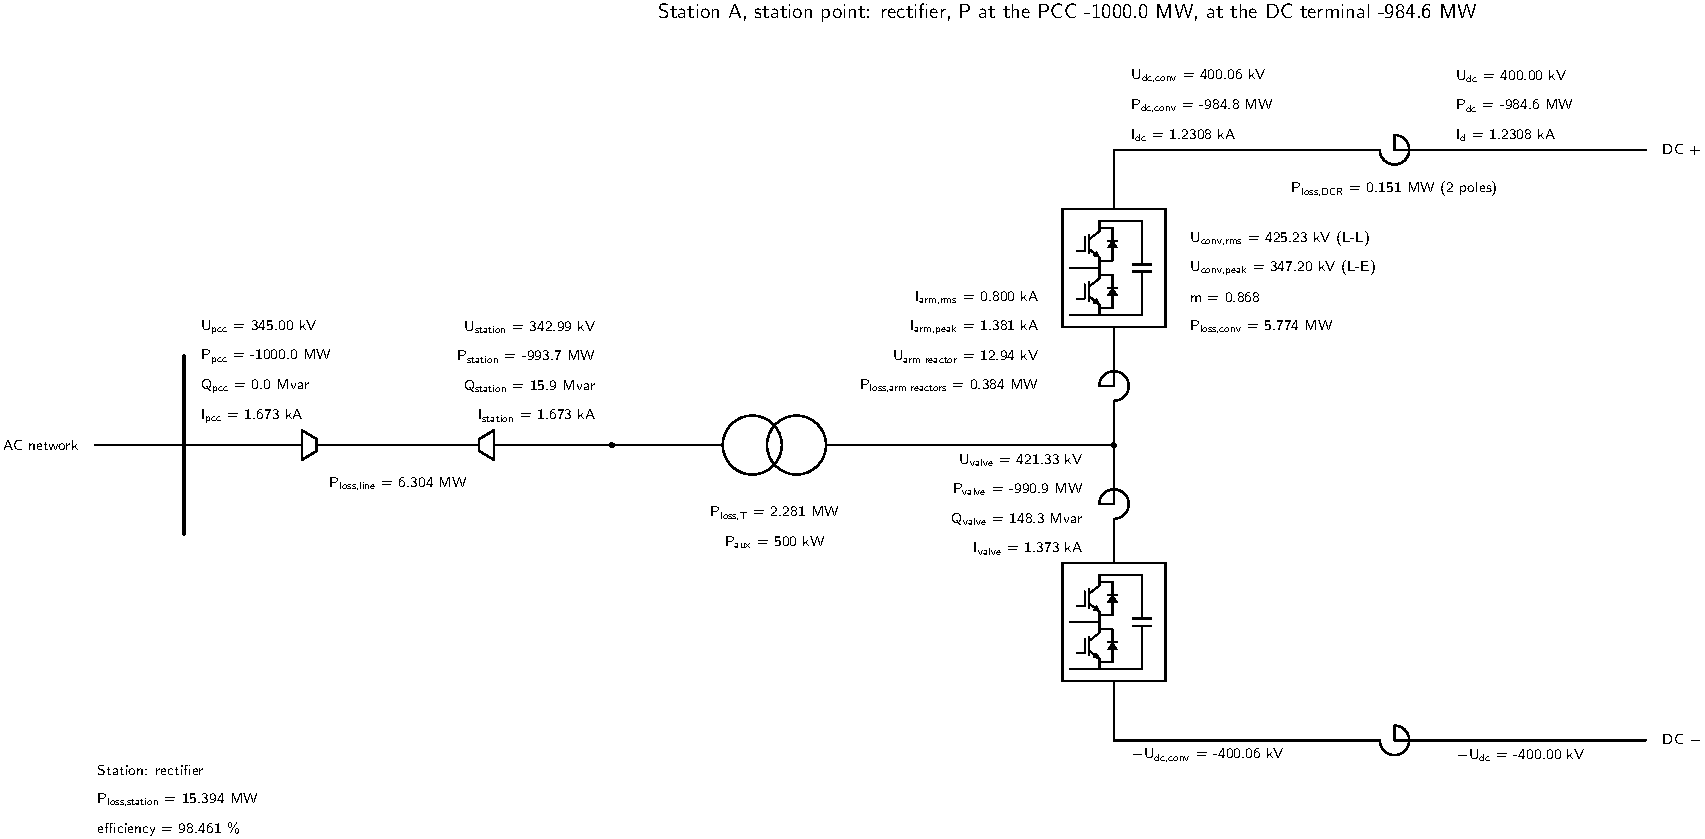
\includegraphics[width=\linewidth]{station/fig/loadflow_station.pdf}
  \caption{Single-line diagram of the example station with the results of Table~\ref{tab:station-chain}}
  \label{fig:station-sld}
\end{figure}

Table~\ref{tab:station-procedures} compares the two solution procedures of Section~\ref{sec:station-procedures}.
The DC power of the first row, given at the DC terminal, reproduces the PCC power after 4 secant iterations. The
third row is an inverter with $P_{dc} = 990$\,MW.

\begin{table}[!ht]
  \centering
  \small
  \begin{tabular}{@{}l r r r r r@{}}
    \toprule
    \textbf{Power given} & \multicolumn{1}{c}{\textbf{$P_{pcc}$ [MW]}} & \multicolumn{1}{c}{\textbf{$P_{dc}$ [MW]}}
      & \multicolumn{1}{c}{\textbf{$I_d$ [kA]}} & \multicolumn{1}{c}{\textbf{$U_{dpe\_conv}$ [kV]}}
      & \multicolumn{1}{c}{\textbf{Iterations}} \\
    \midrule
    \tablerows{station/fig/procedures_table}
    \bottomrule
  \end{tabular}
  \caption{Active power given at the PCC and at the station DC terminal; iterations of the secant method}
  \label{tab:station-procedures}
\end{table}
\FloatBarrier


% =============================================================
%  Chapter -- Converter
%  The chapter heading and introduction; one file per subsection:
%    ac-side.tex      internal voltage, modulation index, arm voltages
%                     and currents, third harmonic, limits, DC side
%    losses.tex       loss models percent_losses and detailed
%    capacitors.tex   submodule capacitor voltage ripple, inner
%                     modulation index
%    example.tex      worked example (Figure arm waveforms; Tables
%                     losses, capacitors)
%  Figures and tables: fig/, generated by fig/converter_example.py from
%  tools/example_data.py (converter at the operating point of the station
%  example, Section 4.4).
%  Sources: [1] hvdc_lf, src/hvdc_lf/components/converter, arm_reactor.
% =============================================================
\section{Converter}
\label{sec:converter}

The converter is a half-bridge MMC: three phase legs, each with an upper and a lower arm of $N$ submodules and one
arm reactor. Its input is the valve-side voltage $U_{valve}$, the active and reactive power $P_{ac}$, $Q_{ac}$ at the
valve terminals (from the transformer) and the DC voltage $U_{dc}$ across its terminals (from the DC side); its
output is the DC power, the internal voltage, the arm quantities, the losses and the limit checks. The model assumes
balanced operation without circulating current and submodules of equal capacitor voltage within an arm. The arm
reactors are a component of their own, the semiconductors as well (Section~\ref{sec:thermal}).

\subsection{Internal Voltage and Arm Quantities}
\label{sec:converter-arm}

\subsubsection{Internal voltage and modulation index}

The upper and lower arm reactors of a phase act in parallel for the AC current, so the equivalent reactance per
phase is $X = \omega \cdot L_{arm} / 2$. With the valve-side phase voltage $U_{ph} = U_{valve} / \sqrt{3}$ as phase
reference, the AC current towards the grid and the internal voltage behind the arm reactors are
\begin{equation}
  \underline{I} = \frac{\left( P_{ac} + \mathrm{j} \cdot Q_{ac} \right)^{*}}{3 \cdot U_{ph}} , \qquad
  \underline{E} = U_{ph} + \mathrm{j} \cdot X \cdot \underline{I} , \qquad
  U_{conv} = \sqrt{3} \cdot |\underline{E}| .
\end{equation}
The arm reactance carries no active power; it absorbs $Q_{arm} = 3 \cdot X \cdot I^2$. The modulation index is the
peak phase voltage in per unit of half the DC voltage:
\begin{equation}
  m = \frac{2 \cdot \sqrt{2} \cdot U_{conv}}{\sqrt{3} \cdot U_{dc}} .
\end{equation}

\subsubsection{Arm voltages and currents}

Over one period, with $e(t) = \sqrt{2} \cdot |\underline{E}| \cdot \cos(\omega t)$ and the AC current $i_{ac}(t)$,
the arms of phase a carry
\begin{align}
  u_{upper}(t) &= \frac{U_{dc}}{2} - \left( e(t) + e_3(t) \right) , &
  i_{upper}(t) &= -\frac{I_{dc}}{3} - \frac{i_{ac}(t)}{2} , \\
  u_{lower}(t) &= \frac{U_{dc}}{2} + \left( e(t) + e_3(t) \right) , &
  i_{lower}(t) &= -\frac{I_{dc}}{3} + \frac{i_{ac}(t)}{2} ,
\end{align}
with the arm currents in their physical direction (upper arm towards the positive terminal) and $I_{dc} > 0$ into
the positive terminal (inverter). Each arm carries a third of the DC current and half of the AC current:
\begin{equation}
  I_{arm\_rms} = \sqrt{\left( \frac{I_{dc}}{3} \right)^2 + \left( \frac{I_{ac}}{2} \right)^2} , \qquad
  I_{arm\_peak} = \frac{|I_{dc}|}{3} + \frac{\sqrt{2} \cdot I_{ac}}{2} .
\end{equation}
The arm reactor losses are $P_{loss\_arm} = 6 \cdot R_{arm} \cdot I_{arm\_rms}^2$. The inserted submodules of an arm
follow its voltage, $n_{ins}(t) = u_{arm}(t) / u_{sm}$, bounded by 0 and $N$.

\subsubsection{Third harmonic injection}

With third harmonic injection the arm voltages contain the zero-sequence component
$e_3(t) = -\tfrac{\sqrt{2} \cdot |\underline{E}|}{6} \cdot \cos(3 \omega t)$. It cancels between the phases and does
not change the AC side; it lowers the peak of $e + e_3$ to $\sqrt{3}/2$ of the fundamental peak. The peak factor is
$k_3 = 1$ without and $k_3 = \sqrt{3}/2$ with injection.

\subsubsection{Limits}

A half-bridge arm cannot produce a negative voltage, and its voltage cannot exceed the sum of its capacitor
voltages:
\begin{equation}
  k_3 \cdot m \le 1 , \qquad
  U_{arm\_max} = \frac{U_{dc}}{2} \cdot \left( 1 + k_3 \cdot m \right) \le N \cdot u_{sm} .
\end{equation}
The highest modulation index at a given DC voltage is therefore
$m_{max} = \min\left( 1, \, 2 \cdot N \cdot u_{sm} / U_{dc} - 1 \right) / k_3$. An exceeded limit is a warning of
the result; the calculation is not stopped. The reactive power the converter can provide at a given active power is
the circle $|\underline{E}| \le E_{max}$ in the $PQ$ plane, with centre $Q = -U_{valve}^2 / X$ and radius
$U_{valve} \cdot E_{max} / X$, $E_{max} = m_{max} \cdot \sqrt{3} \cdot U_{dc} / (2 \cdot \sqrt{2})$ line-to-line.

\subsubsection{DC side}

The DC power is the AC power plus the losses, and the DC current follows from the DC voltage:
\begin{equation}
  P_{dc} = P_{ac} + P_{loss\_cv} , \qquad I_{dc} = \frac{P_{dc}}{U_{dc}} ,
\end{equation}
both in the convention of Section~\ref{sec:conventions} ($P_{dc} < 0$ for a rectifier). The converter can also be
calculated with $P_{dc}$ or $I_{dc}$ given; then $P_{ac} = P_{dc} - P_{loss\_cv}(P_{ac})$ is iterated to a change
below $10^{-10}$ of $|P_{dc}|$.

\subsection{Losses}
\label{sec:converter-losses}

\subsubsection{Loss model \texttt{percent\_losses}}

The losses are a fixed share of the throughput plus the arm reactors:
$P_{loss\_cv} = \tfrac{p_{loss}}{100} \cdot |P_{ac}| + 6 \cdot R_{arm} \cdot I_{arm\_rms}^2$.

\subsubsection{Loss model \texttt{detailed}}

The detailed model calculates the semiconductor losses from the arm voltages and currents of one period, sampled at
$M = 360$ points. In every arm the current flows through one switch position of each submodule: through the upper
switch position (T1/D1) of an inserted submodule and through the lower switch position (T2/D2) of a bypassed one. In
the upper position the diode D1 conducts the charging current ($-i_{arm} > 0$, into the capacitor) and the IGBT T1
the discharging current; in the lower position T2 conducts the charging and D2 the discharging current. With
$n_{par}$ modules in parallel at each switch position, the current shares equally and the conduction losses of one
switch position are, with the on-state model $v = v_0 + r \cdot i$ of Section~\ref{sec:semiconductor},
\begin{equation}
  p_{cond}(i) = v_0 \cdot |i| + \frac{r \cdot i^2}{n_{par}} .
\end{equation}
The conduction losses of an arm are the mean over the period of
\begin{equation}
  n_{ins}(t) \cdot p_{ins}\!\left( i_{arm}(t) \right) + \left( N - n_{ins}(t) \right) \cdot p_{byp}\!\left( i_{arm}(t) \right) ,
\end{equation}
with $p_{ins}$ the diode (charging) or the IGBT (discharging) of the inserted position and $p_{byp}$ the IGBT
(charging) or the diode (discharging) of the bypassed position. The switching losses scale the datasheet energies
linearly with the submodule voltage and the current:
\begin{equation}
  P_{sw\_arm} = N \cdot f_{sw} \cdot \left( E_{on} + E_{off} + E_{rec} \right) \cdot \frac{u_{sm}}{U_{sw\_ref}}
                \cdot \frac{\overline{|i_{arm}|}}{I_{sw\_ref}} ,
\end{equation}
with $f_{sw}$ the average switching frequency of a submodule and $\overline{|i_{arm}|}$ the mean of the absolute arm
current. Each switching event at a switch position is shared by its $n_{par}$ modules, so $P_{sw\_arm}$ does not
depend on $n_{par}$; the slope part of the conduction losses decreases with $1/n_{par}$ and the threshold part does
not. Constant losses per submodule $p_{sm}$ (gate unit supply, capacitor, bleeder resistor) add $6 \cdot N \cdot p_{sm}$.
The converter losses are
\begin{equation}
  P_{loss\_cv} = \sum_{6\ \mathrm{arms}} \left( P_{cond\_arm} + P_{sw\_arm} \right) + 6 \cdot N \cdot p_{sm}
                 + 6 \cdot R_{arm} \cdot I_{arm\_rms}^2 .
\end{equation}
The upper and lower arms of a phase have the same losses; the three phases are equal.

\subsubsection{Loss iteration}

The arm currents contain $I_{dc} / 3$, and $I_{dc} = (P_{ac} + P_{loss\_cv}) / U_{dc}$ depends on the losses. The
losses are found by a fixed-point iteration on $P_{loss\_cv}$, starting from zero, until the change is below
$10^{-12} \cdot \max(1, |P_{ac}|)$.

\subsection{Submodule Capacitors}
\label{sec:converter-capacitors}

\subsubsection{Capacitor voltage ripple}

With the submodule capacitance $C_{sm}$ given, the variation of the capacitor voltages over one period is calculated.
An arm takes the power $p(t) = -u_{arm}(t) \cdot i_{arm}(t)$ (charging current). Its mean is the share of the
losses of the arm; the remainder charges and discharges the inserted capacitors. The energy variation of an arm is
\begin{equation}
  \Delta W(t) = \int_0^t \left( p(t') - \overline{p} \right) \mathrm{d}t' ,
\end{equation}
evaluated over the $M$ samples. Around the stored energy $W_0 = N \cdot C_{sm} \cdot u_{sm}^2 / 2$ of an arm,
with the capacitors of an arm balanced and $u_{sm}$ their average voltage,
\begin{equation}
  W(t) = W_0 + \Delta W(t) - \overline{\Delta W} , \qquad
  u_c(t) = \sqrt{\frac{2 \cdot W(t)}{N \cdot C_{sm}}} .
\end{equation}
The result gives the stored energy of the six arms, per MV$\cdot$A of $|\underline{S}_{ac}|$, the peak-to-peak
energy variation of an arm, the lowest and highest capacitor voltage and the ripple in per cent of $u_{sm}$. The
ripple does not change $P$ and $Q$ of the load flow. A capacitance so small that $W(t) \le 0$ is rejected.

\subsubsection{Inner modulation index}

The inner modulation index relates the voltage an arm produces to the sum of its capacitor voltages:
\begin{equation}
  a = \max_t \frac{u_{arm}(t)}{N \cdot u_c(t)} \le 1 ,
\end{equation}
with $u_c = u_{sm}$ when no capacitance is given, $a = U_{arm\_max} / (N \cdot u_{sm})$. The margin
$\min_t \left( N \cdot u_c(t) - u_{arm}(t) \right)$ is the voltage reserve of the arm; $a > 1$ is a warning. The
capacitor ripple shifts $a$ in either direction: $a$ rises if the capacitors of an arm are below average when the
arm voltage is highest and falls if they are above average, depending on the operating point.

\subsection{Worked Example}
\label{sec:converter-example}

The converter of the example station at its operating point of Section~\ref{sec:station-example} has
$U_{valve} = \cvUv$\,kV, $P_{ac} = \cvP$\,MW, $Q_{ac} = \cvQ$\,Mvar and $U_{dc} = \cvUdc$\,kV. The arm
currents are $I_{arm\_rms} = \cvIrms$\,kA and $I_{arm\_peak} = \cvIpk$\,kA. Figure~\ref{fig:converter-arm} shows the arm voltages,
the arm currents and the capacitor voltages of phase a over one period; Table~\ref{tab:converter-losses} gives the
losses of the detailed model and Table~\ref{tab:converter-capacitors} the capacitor quantities.

\begin{figure}[!ht]
  \centering
  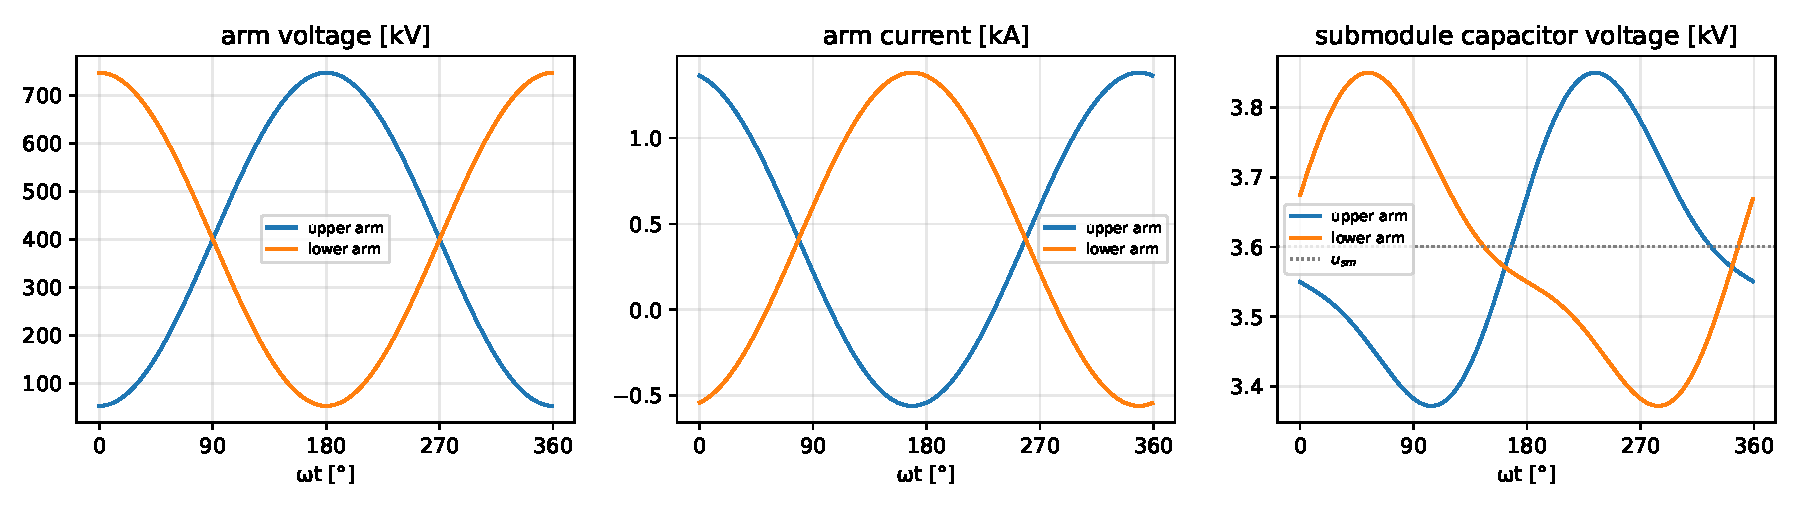
\includegraphics[width=\linewidth]{converter/fig/arm_waveforms.pdf}
  \caption{Arm voltages, arm currents and submodule capacitor voltages of phase a over one period, converter of the
           example at $P_{ac} = \cvP$\,MW (rectifier)}
  \label{fig:converter-arm}
\end{figure}

\begin{table}[!ht]
  \centering
  \small
  \begin{tabular}{@{}l r r@{}}
    \toprule
    \textbf{Part} & \multicolumn{1}{c}{\textbf{MW}} & \multicolumn{1}{c}{\textbf{\% of $|P_{ac}|$}} \\
    \midrule
    \tablerows{converter/fig/losses_table}
    \bottomrule
  \end{tabular}
  \caption{Converter losses of the example, loss model \texttt{detailed}, two modules in parallel}
  \label{tab:converter-losses}
\end{table}

\begin{table}[!ht]
  \centering
  \small
  \begin{tabular}{@{}l r l@{}}
    \toprule
    \textbf{Quantity} & \multicolumn{1}{c}{\textbf{Value}} & \multicolumn{1}{c}{\textbf{Unit}} \\
    \midrule
    \tablerows{converter/fig/capacitor_table}
    \bottomrule
  \end{tabular}
  \caption{Modulation and submodule capacitor quantities of the example, $C_{sm} = 3.7$\,mF}
  \label{tab:converter-capacitors}
\end{table}
\FloatBarrier


% =============================================================
%  Chapter -- Semiconductor and Cooling
%  The chapter heading and introduction; one file per subsection:
%    semiconductor.tex  module data, on-state model fitted to the
%                       datasheet (Table onstate), ratings
%    die-losses.tex     losses of the four dies of a submodule
%    cooling.tex        cold plate and water path
%    junction.tex       Foster model, periodic steady state
%    example.tex        worked example (Tables modules, dies, flow;
%                       Figure junction waveforms)
%  Figures and tables: fig/, generated by fig/thermal_example.py from
%  tools/example_data.py.
%  Sources: [1] hvdc_lf, src/hvdc_lf/components/semiconductor,
%  components/converter/calc.py (die_losses, periodic_rise, thermal);
%  [2] CM1000HG-130XA datasheet; [3] Dittus and Boelter.
% =============================================================
\section{Semiconductor and Cooling}
\label{sec:thermal}

The semiconductor is the IGBT module with its anti-parallel diode at one switch position of a submodule. Its data
--- ratings, on-state model, switching energies and thermal model --- are a component of their own, taken from the
datasheet at one junction temperature. The converter links to it and adds the number of modules in parallel, the
switching frequency and the cold plate. With these data the converter calculates the losses of
Section~\ref{sec:converter-losses} and the junction temperatures of the dies in the periodic steady state of one
period, without time integration.

\subsection{Semiconductor Data}
\label{sec:semiconductor}

The example module is the Mitsubishi Electric CM1000HG-130XA, 6.5\,kV, 1000\,A, with the data at
$T_j = 125\,^{\circ}$C~[2]. The on-state voltage of IGBT and diode is modelled per module as
\begin{equation}
  v_{CE} = v_{0\_igbt} + r_{igbt} \cdot i_C , \qquad v_{EC} = v_{0\_diode} + r_{diode} \cdot i_E ,
\end{equation}
fitted through the datasheet values at 1000\,A ($V_{CE\_sat} = 3.25$\,V, $V_{EC} = 2.80$\,V, typical, $T_j = 125\,^{\circ}$C)
and the typical output characteristics at 500\,A. This gives $v_{0\_igbt} = 1.45$\,V, $r_{igbt} = 1.80$\,m$\Omega$,
$v_{0\_diode} = 1.60$\,V and $r_{diode} = 1.20$\,m$\Omega$. Table~\ref{tab:onstate} compares the model with the
datasheet: the deviation is at most 0.1\,V from 250\,A to 1000\,A, which covers the module currents of the converter
(up to 0.69\,kA per module in the example), and reaches 0.5\,V at 2000\,A. The points other than 1000\,A are read
from the characteristics with an accuracy of about $\pm 0.1$\,V.

\begin{table}[!ht]
  \centering
  \small
  \begin{tabular}{@{}l r r r r@{}}
    \toprule
    \textbf{Device} & \multicolumn{1}{c}{\textbf{$i$ [kA]}} & \multicolumn{1}{c}{\textbf{Datasheet [V]}}
      & \multicolumn{1}{c}{\textbf{Model [V]}} & \multicolumn{1}{c}{\textbf{Deviation [V]}} \\
    \midrule
    \tablerows{thermal/fig/onstate_table}
    \bottomrule
  \end{tabular}
  \caption{On-state model of the CM1000HG-130XA against the datasheet, $T_j = 125\,^{\circ}$C~[2]}
  \label{tab:onstate}
\end{table}

The switching energies per pulse are those of the datasheet at $V_{CC} = 3600$\,V, $I_C = 1000$\,A,
$R_{G\_on} = 4.3\,\Omega$, $R_{G\_off} = 39\,\Omega$, $L_s = 150$\,nH and $T_j = 125\,^{\circ}$C, as defined in
IEC 60747: $E_{on} = 11.0$\,J, $E_{off} = 7.5$\,J, $E_{rec} = 5.1$\,J~[2]. The converter scales them linearly with
voltage and current (Section~\ref{sec:converter-losses}). The datasheet curves of the energies against current are
not linear; below 1000\,A the linear scaling gives lower energies than the curves.

The thermal data are $R_{th\_jc} = 10.0$\,K/kW (IGBT) and 16.0\,K/kW (diode), maximum values, the contact resistance
case to heat sink $R_{th\_cs} = 5.0$\,K/kW per module (typical, grease $\lambda = 1$\,W/(m$\cdot$K), 80\,$\mu$m), the
highest operating junction temperature $T_{jop} = 150\,^{\circ}$C, and the Foster model of the transient thermal
impedance junction to case, the same for IGBT and diode:
\begin{equation}
  Z_{th\_jc}(t) = R_{th\_jc} \cdot \sum_{i=1}^{4} r_i \cdot \left( 1 - \mathrm{e}^{-t/\tau_i} \right) ,
\end{equation}
with $r_i = 0.0096$, 0.1893, 0.4044, 0.3967 and $\tau_i = 0.1$\,ms, 5.8\,ms, 60.2\,ms, 351.2\,ms~[2].

With the ratings given, the converter warns when the highest submodule capacitor voltage reaches the blocking
voltage $V_{CES}$ and when the peak current per module $I_{arm\_peak} / n_{par}$ exceeds the rated collector current
$I_C$. With one module per switch position the example exceeds $I_C$ (1.38\,kA); with two it does not.

\subsection{Losses of the Dies}
\label{sec:die-losses}

The junction temperatures need the losses of each of the four dies T1, D1, T2, D2 of a submodule separately. The
losses of Section~\ref{sec:converter-losses} are assigned to the dies of the average submodule of an arm, which is
inserted for the share $n_{ins}(t) / N$ of the time. With the current of one module $i_m = |i_{arm}| / n_{par}$,
\begin{equation}
  p_{cond\_igbt} = v_{0\_igbt} \cdot i_m + r_{igbt} \cdot i_m^2 , \qquad
  p_{cond\_diode} = v_{0\_diode} \cdot i_m + r_{diode} \cdot i_m^2 ,
\end{equation}
and the switching powers of one module
\begin{equation}
  p_{sw\_igbt} = f_{sw} \cdot (E_{on} + E_{off}) \cdot \frac{u_{sm}}{U_{sw\_ref}} \cdot \frac{i_m}{I_{sw\_ref}} , \qquad
  p_{sw\_diode} = f_{sw} \cdot E_{rec} \cdot \frac{u_{sm}}{U_{sw\_ref}} \cdot \frac{i_m}{I_{sw\_ref}} ,
\end{equation}
the dies of one module carry, for each sample of the period,
\begin{center}
  \begin{tabular}{@{}l l l@{}}
    \toprule
    & \textbf{Charging current ($-i_{arm} > 0$)} & \textbf{Discharging current} \\
    \midrule
    T1 & 0 & $\frac{n_{ins}}{N} \cdot p_{cond\_igbt} + p_{sw\_igbt}$ \\
    D1 & $\frac{n_{ins}}{N} \cdot p_{cond\_diode} + p_{sw\_diode}$ & 0 \\
    T2 & $\left( 1 - \frac{n_{ins}}{N} \right) \cdot p_{cond\_igbt} + p_{sw\_igbt}$ & 0 \\
    D2 & 0 & $\left( 1 - \frac{n_{ins}}{N} \right) \cdot p_{cond\_diode} + p_{sw\_diode}$ \\
    \bottomrule
  \end{tabular}
\end{center}
With charging current the IGBT T2 switches and the diode D1 recovers; with discharging current T1 switches and D2
recovers. The sum over the dies of all $6 \cdot N \cdot n_{par}$ modules equals the conduction and switching losses
of the converter. The upper and lower arms of a phase are calculated both; the temperatures are reported for the
hotter one.

\subsection{Cold Plate and Water Path}
\label{sec:cooling}

Each submodule sits on one liquid-cooled cold plate. The heat capacity of the plate and the water keeps the heat sink
temperature constant over one period, so the cooling path is calculated with the mean losses of the period. The
$n_{par}$ modules in parallel at a switch position have parallel water paths with the flow $Q_w / n_{par}$ each,
$Q_w$ the flow per cold plate. Along one path the water passes the module of one switch position and then the module
of the other (T1/D1 first in the example), so the second module sees water warmed by the first.

The thermal resistance heat sink to water under one module is one value of the converter design, $R_{th\_hw\_ref}$
at the reference flow $Q_{ref}$, with the flow dependence of the heat transfer coefficient in turbulent flow~[3]:
\begin{equation}
  R_{th\_hw}(Q_w) = R_{th\_hw\_ref} \cdot \left( \frac{Q_{ref}}{Q_w} \right)^{0.8} .
\end{equation}
The example uses $R_{th\_hw\_ref} = 6$\,K/kW at $Q_{ref} = 10$\,l/min, a value to be replaced by the data of the
cold plate. For module $j$ along the path with the mean losses $P_j$ (IGBT and diode),
\begin{align}
  \Delta T_{w\_j} &= \frac{P_j}{\rho \cdot c_p \cdot Q_w / n_{par}} , &
  T_{w\_j} &= T_{w\_in} + \sum_{i<j} \Delta T_{w\_i} + \frac{\Delta T_{w\_j}}{2} , \\
  T_{hs\_j} &= T_{w\_j} + P_j \cdot R_{th\_hw}(Q_w) , &
  T_{case\_j} &= T_{hs\_j} + P_j \cdot R_{th\_cs} ,
\end{align}
with $\rho \cdot c_p = 4.13$\,kJ/(l$\cdot$K) for water at about 50\,$^{\circ}$C ($988\,\mathrm{kg/m^3} \cdot
4.18\,\mathrm{kJ/(kg \cdot K)}$) and $T_{w\_j}$ the mean water temperature along the module. The water inlet
temperature $T_{w\_in}$ (default 50\,$^{\circ}$C) and the flow per cold plate $Q_w$ (default $Q_{ref}$) are part of the
operating point. The water outlet temperature follows from the losses of the cold plate,
$T_{w\_out} - T_{w\_in} = P_{plate} / (\rho \cdot c_p \cdot Q_w)$.

\subsection{Junction Temperature}
\label{sec:junction}

The junction temperature of a die is the case temperature plus the rise across the Foster network of
Section~\ref{sec:semiconductor}, driven by the die losses $p(t)$ of Section~\ref{sec:die-losses}. The losses are
periodic, so the temperatures are as well, and the network is linear. Each Foster element $R_i = r_i \cdot R_{th\_jc}$,
$\tau_i$ is solved exactly for losses that are constant within each of the $M$ samples of length
$\Delta t = 1 / (f \cdot M)$:
\begin{equation}
  \vartheta_i(n+1) = a_i \cdot \vartheta_i(n) + (1 - a_i) \cdot R_i \cdot p(n) , \qquad
  a_i = \mathrm{e}^{-\Delta t / \tau_i} .
\end{equation}
The periodic steady state requires $\vartheta_i(M) = \vartheta_i(0)$, which gives the start value directly:
\begin{equation}
  \vartheta_i(0) = \frac{\sum_{n=0}^{M-1} a_i^{M-1-n} \cdot (1 - a_i) \cdot R_i \cdot p(n)}{1 - a_i^M} .
\end{equation}
One pass over the period from this start value gives the temperature rise; no transient has to settle. The
junction temperature is
\begin{equation}
  T_j(n) = T_{case} + \sum_{i=1}^{4} \vartheta_i(n) .
\end{equation}
Its mean over the period is $T_{case} + R_{th\_jc} \cdot \overline{p}$. The two short time constants (0.1\,ms and
5.8\,ms) set the ripple over the 16.7\,ms period at 60\,Hz; the long ones (60\,ms, 351\,ms) mainly add to the mean.
A junction temperature above $T_{jop}$ is a warning.

The model holds the loss data at the junction temperature of the semiconductor data (125\,$^{\circ}$C); the
dependence of the losses on the calculated junction temperature is not iterated. $R_{th\_jc}$ is a maximum value of
the datasheet, so the junction temperatures are upper values for the given losses.

\subsection{Worked Example}
\label{sec:thermal-example}

At the converter operating point of Section~\ref{sec:converter-example}, with $T_{w\_in} = 50\,^{\circ}$C and
$Q_w = 10$\,l/min per cold plate, the cold plate carries $\thPplate$\,kW and the water leaves it at
$\thTout\,^{\circ}$C. Table~\ref{tab:thermal-modules} gives the temperatures along one water path and
Table~\ref{tab:thermal-dies} the losses and junction temperatures of the dies, for the \thArm{} arm. The hottest die
is \thHot{} at $\thTjmax\,^{\circ}$C. Figure~\ref{fig:junction} shows the losses and junction temperatures of the
four dies over one period.

\begin{table}[!ht]
  \centering
  \small
  \begin{tabular}{@{}l r r r r r@{}}
    \toprule
    \textbf{Module} & \multicolumn{1}{c}{\textbf{Order}} & \multicolumn{1}{c}{\textbf{$P_j$ [kW]}}
      & \multicolumn{1}{c}{\textbf{$T_w$ [$^{\circ}$C]}} & \multicolumn{1}{c}{\textbf{$T_{hs}$ [$^{\circ}$C]}}
      & \multicolumn{1}{c}{\textbf{$T_{case}$ [$^{\circ}$C]}} \\
    \midrule
    \tablerows{thermal/fig/modules_table}
    \bottomrule
  \end{tabular}
  \caption{Temperatures along one water path of the cold plate, example at $T_{w\_in} = 50\,^{\circ}$C,
           $Q_w = 10$\,l/min}
  \label{tab:thermal-modules}
\end{table}

\begin{table}[!ht]
  \centering
  \small
  \begin{tabular}{@{}l r r r r r@{}}
    \toprule
    \textbf{Die} & \multicolumn{1}{c}{\textbf{$\overline{p}$ [kW]}} & \multicolumn{1}{c}{\textbf{$p_{max}$ [kW]}}
      & \multicolumn{1}{c}{\textbf{$\overline{T_j}$ [$^{\circ}$C]}} & \multicolumn{1}{c}{\textbf{$T_{j\_max}$ [$^{\circ}$C]}}
      & \multicolumn{1}{c}{\textbf{$\Delta T_{j\_pp}$ [K]}} \\
    \midrule
    \tablerows{thermal/fig/dies_table}
    \bottomrule
  \end{tabular}
  \caption{Losses and junction temperatures of the dies of one module per switch position, example as in
           Table~\ref{tab:thermal-modules}}
  \label{tab:thermal-dies}
\end{table}

\begin{figure}[!ht]
  \centering
  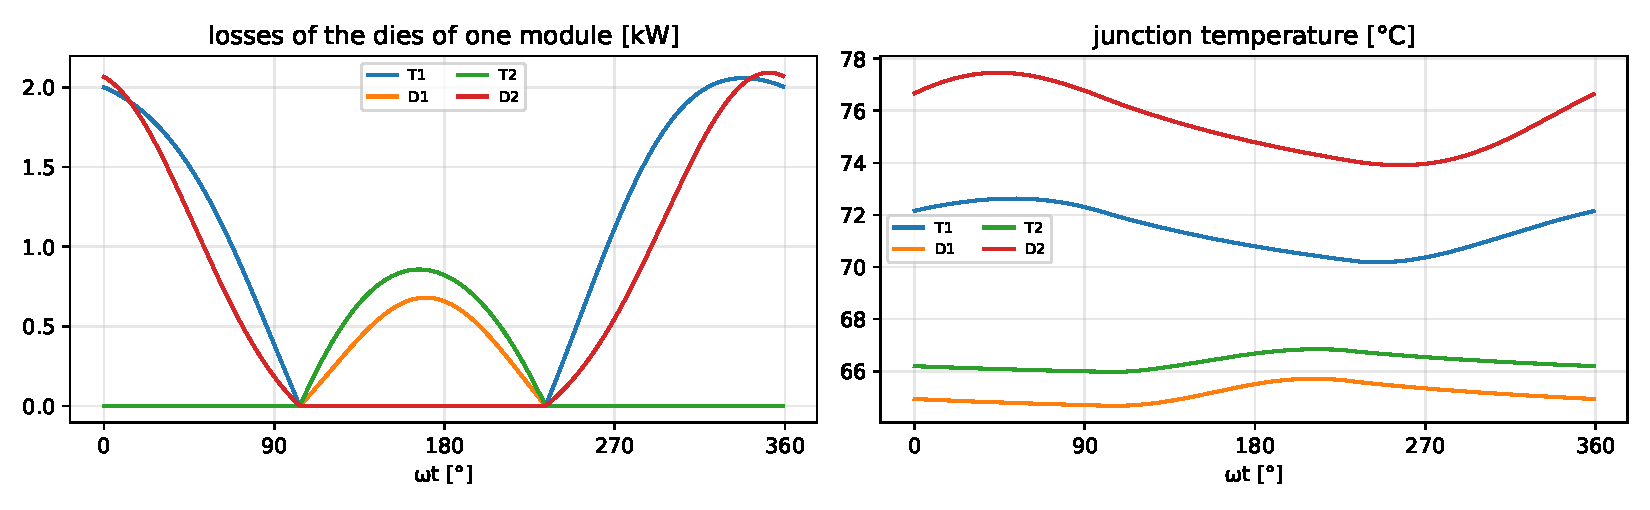
\includegraphics[width=\linewidth]{thermal/fig/junction_waveforms.pdf}
  \caption{Losses and junction temperatures of the dies over one period, example as in Table~\ref{tab:thermal-modules}}
  \label{fig:junction}
\end{figure}

Table~\ref{tab:thermal-flow} gives the highest junction temperature against the water flow per cold plate and the
inlet temperature. The inlet temperature adds one to one; halving the flow from 10\,l/min to 5\,l/min raises the
highest junction temperature by 8.3\,K.

\begin{table}[!ht]
  \centering
  \small
  \begin{tabular}{@{}r r r r@{}}
    \toprule
    \multicolumn{1}{c}{\textbf{$Q_w$ [l/min]}} & \multicolumn{1}{c}{\textbf{$T_{w\_in} = 40\,^{\circ}$C}}
      & \multicolumn{1}{c}{\textbf{50\,$^{\circ}$C}} & \multicolumn{1}{c}{\textbf{60\,$^{\circ}$C}} \\
    \midrule
    \tablerows{thermal/fig/flow_table}
    \bottomrule
  \end{tabular}
  \caption{Highest junction temperature in $^{\circ}$C against water flow per cold plate and inlet temperature}
  \label{tab:thermal-flow}
\end{table}
\FloatBarrier


% =============================================================
%  Chapter -- DC Line
%  Subsections: Resistance, Voltage drop and losses, Current for a
%  given power, Worked example.
%  Values: link/fig/link_values.tex (generated by link/fig/link_example.py
%  from tools/example_data.py).
%  Sources: [1] hvdc_lf, src/hvdc_lf/components/dc_line/calc.py.
% =============================================================
\section{DC Line}
\label{sec:dc-line}

The DC line connects the DC terminals of the two stations of a link. One pole conductor is calculated; a pole may
consist of $n_{sub}$ conductors in parallel. The line is modelled by its DC resistance; inductance and capacitance
have no effect in the steady state. Both pole conductors carry the same current $I_d$ (balanced operation, no current
in the return path), so the line losses of the link are $n_{pc}$ times those of one pole conductor, $n_{pc} = 2$.

\subsection{Resistance}

The conductor data give the DC resistance per kilometre $R'_{ref}$ at the reference temperature $T_{ref}$ and its
temperature coefficient $\alpha$. The resistance of one pole at the conductor temperature $T$ is
\begin{equation}
  R_{pole}(T) = \frac{R'_{ref} \cdot \left( 1 + \alpha \cdot (T - T_{ref}) \right)}{n_{sub}} \cdot l .
\end{equation}
The conductor temperature is an operating value; without one the design temperature $T_{design}$ of the line is
used.

\subsection{Voltage Drop and Losses}

With the voltage $U_{send}$ pole-to-ground at the sending end (rectifier DC terminal) and the pole current $I_d$,
\begin{equation}
  U_{recv} = U_{send} - R_{pole} \cdot I_d , \qquad
  P_{send} = U_{send} \cdot I_d , \qquad
  P_{recv} = U_{recv} \cdot I_d , \qquad
  P_{loss\_line} = R_{pole} \cdot I_d^2 .
\end{equation}
These powers are per pole and taken as positive in the direction of the power flow. The loading of the line is
$I_d / (n_{sub} \cdot I_r)$ with the rated current $I_r$ of one conductor, when it is given.

\subsection{Current for a Given Power}

For a power given at the sending end, $I_d = P_{send} / U_{send}$. For a power given at the receiving end,
$P_{recv} = (U_{send} - R_{pole} \cdot I_d) \cdot I_d$ is a quadratic equation in $I_d$ with the smaller root
\begin{equation}
  I_d = \frac{U_{send} - \sqrt{U_{send}^2 - 4 \cdot R_{pole} \cdot P_{recv}}}{2 \cdot R_{pole}} .
\end{equation}
A real solution exists up to $P_{recv\_max} = U_{send}^2 / (4 \cdot R_{pole})$; a larger power is rejected. The
larger root belongs to operation beyond this maximum, with $U_{recv} < U_{send} / 2$, and is not used.

\subsection{Worked Example}
\label{sec:dc-line-example}

The example line is a 300\,km XLPE cable, 2500\,mm$^2$ copper, one conductor per pole, $R'_{ref} = 0.0072\,\Omega$/km
at 20\,$^{\circ}$C, $\alpha = 0.00393$\,1/K, $I_r = 2.0$\,kA and $T_{design} = 70\,^{\circ}$C. The pole resistance is
$\lkRtwenty\,\Omega$ at 20\,$^{\circ}$C and $\lkRseventy\,\Omega$ at 70\,$^{\circ}$C. At $U_{send} = 400$\,kV and
$I_d = \lkId$\,kA the receiving end voltage is $\lkUinv$\,kV and the losses of both pole conductors are
$\lkLine$\,MW. The maximum power at the receiving end is 15\,480\,MW per pole, about 31 times the power of the example.

% =============================================================
%  Chapter -- Link
%  Subsections: Operating point and direction, DC circuit, Solution
%  procedures, Link totals and checks, Worked example (Table points).
%  Tables and values: fig/points_table.tex, fig/link_values.tex, generated
%  by fig/link_example.py from tools/example_data.py.
%  Sources: [1] hvdc_lf, src/hvdc_lf/link/case.py, link/solver.py.
% =============================================================
\section{Link}
\label{sec:link}

A link consists of two stations A and B, each calculated as in Section~\ref{sec:station}, and the DC line of
Section~\ref{sec:dc-line} between their DC terminals. The link configuration holds the two stations, the DC line and
the topology; the rectifier and the inverter are not part of it. Both stations may have the same design or different
ones.

\subsection{Operating Point and Direction}
\label{sec:link-point}

The operating point of a link gives, at both PCCs, the voltage, frequency, reactive power, tap position and auxiliary
power, the DC voltage $U_{dpe\_rec}$ at the rectifier DC terminal, the conductor temperature and the cooling data of
both converters. The active power is given at exactly one of four points, signed as for a single station:
$P_{pcc\_a}$, $P_{pcc\_b}$ (PCC of station A or B) or $P_{dc\_a}$, $P_{dc\_b}$ (DC terminal of station A or B, all
poles). The station at which the power is given is the rectifier if the power is negative, the inverter if it is
positive; the other station takes the other role. Seen from the power flow, the given point is one of four
references, which select the solution procedure of Section~\ref{sec:link-procedures}, Table~\ref{tab:link-reference}.

\begin{table}[!ht]
  \centering
  \small
  \begin{tabular}{@{}l l l l@{}}
    \toprule
    \textbf{Given} & \multicolumn{1}{c}{\textbf{Sign}} & \multicolumn{1}{c}{\textbf{Rectifier}}
      & \multicolumn{1}{c}{\textbf{Reference}} \\
    \midrule
    $P_{pcc\_a}$ & $< 0$ & A & sending AC \\
    $P_{pcc\_a}$ & $> 0$ & B & receiving AC \\
    $P_{pcc\_b}$ & $< 0$ & B & sending AC \\
    $P_{pcc\_b}$ & $> 0$ & A & receiving AC \\
    $P_{dc\_a}$  & $< 0$ & A & sending DC \\
    $P_{dc\_a}$  & $> 0$ & B & receiving DC \\
    $P_{dc\_b}$  & $< 0$ & B & sending DC \\
    $P_{dc\_b}$  & $> 0$ & A & receiving DC \\
    \bottomrule
  \end{tabular}
  \caption{Rectifier and power reference from the point and the sign of the given active power}
  \label{tab:link-reference}
\end{table}

\subsection{DC Circuit}
\label{sec:link-dc}

The DC circuit of one pole runs from the converter terminals of the rectifier through its DC reactor, the DC line
and the DC reactor of the inverter to the converter terminals of the inverter. For the current $I_d$ and the given
$U_{dpe\_rec}$,
\begin{align}
  U_{dpe\_conv\_rec} &= U_{dpe\_rec} + R_{dcr\_rec} \cdot I_d , \\
  U_{dpe\_inv} &= U_{dpe\_rec} - R_{pole} \cdot I_d , \\
  U_{dpe\_conv\_inv} &= U_{dpe\_inv} - R_{dcr\_inv} \cdot I_d ,
\end{align}
with $U_{dpe\_inv}$ the voltage at the inverter DC terminal (line end). The converters see
$U_{dc} = k \cdot U_{dpe\_conv}$ and carry $|P_{dc\_cv}| = k \cdot U_{dpe\_conv} \cdot I_d$ each.

\subsection{Solution Procedures}
\label{sec:link-procedures}

The four procedures use the station chain and the secant search on $P_{pcc}$ of
Section~\ref{sec:station-procedures} for a station whose converter DC power is known. The link secants have the
tolerance $10^{-6}$\,MW and at most 50 iterations.

\paragraph{Sending AC.} $P_{pcc}$ of the rectifier is given.
\begin{enumerate}
  \item Rectifier chain with the given $P_{pcc}$ and the fixed point on $U_{dpe\_conv\_rec}$ of
        Section~\ref{sec:station-procedures}, giving $I_d$.
  \item DC circuit, giving $U_{dpe\_conv\_inv}$.
  \item Inverter: secant on its $P_{pcc}$ until its converter DC power is $k \cdot U_{dpe\_conv\_inv} \cdot I_d$.
\end{enumerate}

\paragraph{Sending DC.} $P_{dc}$ at the rectifier DC terminal is given.
\begin{enumerate}
  \item $I_d = |P_{dc}| / (n_{conv} \cdot k \cdot U_{dpe\_rec})$ and the DC circuit, giving both converter voltages.
  \item Rectifier: secant on its $P_{pcc}$ until its converter DC power is $-k \cdot U_{dpe\_conv\_rec} \cdot I_d$.
  \item Inverter: secant as for sending AC, independent of step 2.
\end{enumerate}

\paragraph{Receiving DC.} $P_{dc}$ at the inverter DC terminal is given.
\begin{enumerate}
  \item Secant on $I_d$ until $n_{conv} \cdot k \cdot U_{dpe\_inv}(I_d) \cdot I_d = P_{dc}$, starting from
        $I_d = P_{dc} / (n_{conv} \cdot k \cdot U_{dpe\_rec})$ and 1.01 times that value. This is the receiving end
        current of Section~\ref{sec:dc-line}, solved numerically through the DC circuit.
  \item Both stations as for sending DC.
\end{enumerate}

\paragraph{Receiving AC.} $P_{pcc}$ of the inverter is given.
\begin{enumerate}
  \item Inverter chain with the given $P_{pcc}$ at the converter voltage $U_{dpe\_conv\_inv}$, starting with
        $U_{dpe\_conv\_inv} = U_{dpe\_rec}$, giving $I_d$.
  \item DC circuit with this $I_d$, giving a new $U_{dpe\_conv\_inv}$; repeat from step 1 until the change is below
        $10^{-6}$\,kV.
  \item Rectifier: secant as for sending DC.
\end{enumerate}

\subsection{Link Totals and Checks}
\label{sec:link-totals}

The powers at the DC terminals are the converter DC powers of all converters plus the DC reactor losses of all pole
conductors, both in the sign convention of Section~\ref{sec:conventions}. The link losses and the efficiency are
\begin{equation}
  P_{loss\_link} = -\left( P_{pcc\_rec} + P_{pcc\_inv} \right) , \qquad
  \eta = \frac{P_{pcc\_inv}}{-P_{pcc\_rec}} .
\end{equation}
The losses must equal the sum of the station losses of both stations and the losses of the $n_{pc}$ pole conductors;
a difference above $10^{-3}$\,MW is a warning. The limit warnings of both stations (Section~\ref{sec:station}) are
collected in the link result.

\subsection{Worked Example}
\label{sec:link-example}

Two stations of the design of Table~\ref{tab:example-data} are joined by the cable of
Section~\ref{sec:dc-line-example}, with the station operating point of Section~\ref{sec:example-data} at both PCCs and
$U_{dpe\_rec} = 400$\,kV. With $P_{pcc\_a} = -1000$\,MW station A is the rectifier; $I_d = \lkId$\,kA, the inverter DC
terminal voltage is $\lkUinv$\,kV, the line losses are $\lkLine$\,MW and the link losses $\lkLoss$\,MW, at an
efficiency of $\lkEta$\,\%. Table~\ref{tab:link-points} gives this operating point with the power given at each of
the four points, rows 1 to 4, and two further points. Rows 1 to 4 give the same operating point, with the power taken
from row 1. In row 5 the power at the PCC of station A is positive, so station B is the rectifier; the DC voltage of
400\,kV is then given at station B, and the current and the losses are higher than in row 1 for the same power at
PCC A, because 1000\,MW are now delivered to grid A instead of taken from it. Row 6 is row 1 mirrored: station B takes
1000\,MW from its grid.

\begin{table}[!ht]
  \centering
  \footnotesize
  \setlength{\tabcolsep}{4pt}
  \begin{tabular}{@{}l c r r r r r r r@{}}
    \toprule
    \textbf{Power given} & \multicolumn{1}{c}{\textbf{Rect.}} & \multicolumn{1}{c}{\textbf{$P_{pcc\_a}$}}
      & \multicolumn{1}{c}{\textbf{$P_{dc\_a}$}} & \multicolumn{1}{c}{\textbf{$P_{dc\_b}$}}
      & \multicolumn{1}{c}{\textbf{$P_{pcc\_b}$}} & \multicolumn{1}{c}{\textbf{$I_d$}}
      & \multicolumn{1}{c}{\textbf{Losses}} & \multicolumn{1}{c}{\textbf{Iter.}} \\
    & & \multicolumn{1}{c}{[MW]} & \multicolumn{1}{c}{[MW]} & \multicolumn{1}{c}{[MW]} & \multicolumn{1}{c}{[MW]}
      & \multicolumn{1}{c}{[kA]} & \multicolumn{1}{c}{[MW]} & \\
    \midrule
    \tablerows{link/fig/points_table}
    \bottomrule
  \end{tabular}
  \caption{Link operating points with the active power given at different points, $U_{dpe\_rec} = 400$\,kV,
           $U_{pcc} = 345$\,kV and $Q_{pcc} = 0$ at both stations}
  \label{tab:link-points}
\end{table}
\FloatBarrier

% =============================================================
%  Chapter -- Verification
%  Subsections: Component contracts, Plausibility checks, Thermal model,
%  Test suite.
%  Sources: [1] hvdc_lf, src/hvdc_lf/*/tests, src/hvdc_lf/services
%  (plausibility), examples/*.ipynb.
% =============================================================
\section{Verification}
\label{sec:verification}

The calculation is verified on three levels: contracts that every calculation method of a component must fulfil,
plausibility checks of a calculated operating point, and the automated test suite of \texttt{hvdc\_lf}~[1].

\subsection{Component Contracts}

Every calculation method of a component is tested against the same contract, independent of its model:
\begin{itemize}
  \item power balance of the element: the power at the grid-side port minus the power at the other port equals the
        losses, in the sign convention of Section~\ref{sec:conventions};
  \item losses $\geq 0$ for rectifier and inverter operation;
  \item DC line: $U_{send} - U_{recv} = R_{pole} \cdot I_d$ and $P_{send} - P_{recv} = R_{pole} \cdot I_d^2$; the
        resistance at $T_{ref}$ equals the catalogue value times the length divided by $n_{sub}$, and increases with
        temperature;
  \item converter: no active power in the arm reactance; $I_{dc} = P_{dc} / U_{dc}$; the loss parts add up to the
        converter losses.
\end{itemize}

\subsection{Plausibility Checks}

Each component, the station and the link have a plausibility check that calculates an operating point and tests
physical relations on the result, each with the result pass or FAIL:
\begin{itemize}
  \item \textbf{Converter:} power balance, $I_{dc} = P_{dc}/U_{dc}$, internal voltage and modulation index, higher
        modulation index with more capacitive reactive power, no-load point, arm current RMS value from the waveform
        against $(I_{dc}/3)^2 + (I_{ac}/2)^2$, Kirchhoff's current law at the phase node, each arm absorbing one sixth
        of the losses, the submodule voltage limit, symmetry of the upper and lower arm losses.
  \item \textbf{Station:} operation from the sign of the given power, the given values reached, continuity of
        voltage and power between the elements, balance of each element and of the station,
        $I_d = P_{dc\_cv} / (2 \cdot U_{dpe\_conv})$.
  \item \textbf{Link:} direction from the sign, the given power reached at its point, signs at the four points,
        the DC voltage at the rectifier terminal equal to the line sending end, $U_{dpe\_rec} - U_{dpe\_inv} =
        R_{pole} \cdot I_d$, DC line balance, station balances, link balance, and the same operating point when the
        power is given at each of the other three points (current, both PCC powers and inverter DC voltage within a
        relative $10^{-6}$).
\end{itemize}
The last link check is the one shown in rows 1 to 4 of Table~\ref{tab:link-points}.

\subsection{Thermal Model}

The closed-form periodic steady state of Section~\ref{sec:junction} is compared with a time integration of the same
Foster network: half-sine losses of 2\,kW peak in 360 samples per period at 60\,Hz, $R_{th\_jc} = 10$\,K/kW and the
Foster data of Section~\ref{sec:semiconductor}, integrated over 500 periods from zero. The temperature rise at the
start of the period agrees within a relative $10^{-6}$, the mean rise equals $R_{th\_jc} \cdot \overline{p}$ within
a relative $10^{-3}$, and constant losses give no ripple and the rise $R_{th\_jc} \cdot p$. In the worked example the
mean junction temperatures satisfy $\overline{T_j} = T_{case} + R_{th\_jc} \cdot \overline{p}$
(Table~\ref{tab:thermal-dies}, e.g.\ T1: $62.7 + 10.0 \cdot 0.870 = 71.4\,^{\circ}$C), and the die losses of all
$6 \cdot 240 \cdot 2$ modules add up to 5.557\,MW, the conduction and switching losses of the converter
(Table~\ref{tab:converter-losses}).

\subsection{Test Suite}

The test suite of \texttt{hvdc\_lf} 0.52.0 holds 27 test modules with the contracts above, the plausibility checks,
the solvers of station and link, the catalogue and the database. It gives 460 passed and 2 skipped tests. The
notebooks of the components, the station and the link in \texttt{examples/} run the plausibility checks on the
example data of Section~\ref{sec:example-data}.

% =============================================================
%  References, numbered in order of first citation.
% =============================================================
\section{References}
\label{sec:references}

\begin{enumerate}[label={[\arabic*]}]
  \item American Terawatt, \texttt{hvdc\_lf} --- load flow framework for MMC VSC HVDC stations and links,
        version 0.52.0, repository \texttt{\textasciitilde/Projects/hidt\_claude/hvdc-loadflow}.
  \item Mitsubishi Electric, \emph{CM1000HG-130XA, HVIGBT module, high voltage insulated type}, datasheet
        HVM-1097-E, October 2023.
  \item F.\,W.\ Dittus, L.\,M.\,K.\ Boelter, \emph{Heat transfer in automobile radiators of the tubular type},
        University of California Publications in Engineering, vol.\ 2, no.\ 13, pp.\ 443--461, 1930.
\end{enumerate}


\end{document}
